\section{Resultados finales y experimentación}

\subsection{Preliminares}

Dado que el objetivo general será tratar de estimar los mejores parámetros para nuestro sistema, haremos listado y una breve descripción de ellos.

\begin{itemize}
\item \textit{iters}: Cantidad de veces que itera el método de la potencia. Cuántas más iteraciones se hagan, mayor será la aproximación al autovalor real, pues en teoría el valor debería obtenerse en el límite.

\item \textit{k\_kNN}: Cantidad de vecinos a considerar en el método de los $k$ vecinos más cercanos (\textit{kNN}).

\item \textit{K\_kfold}: Cantidad de grupos (\textit{folds}) en el que vamos a dividir nuestro set de datos en los experimentos, para la aplicación de \textit{K-fold cross validation}

\item \textit{alpha ($\alpha$)}: Cantidad de dimensiones consideradas para el análisis de componentes principales (\textit{PSA}).

\end{itemize}
$ $\newline
Las métricas que utilizaremos para analizar las clasificaciones son las siguientes:

\begin{itemize}

    \item \textit{accuracy}: Imágenes bien clasificadas por sobre el total.

    \item \textit{tp}: True Positive.

    \item \textit{fp}: False Positive.

    \item \textit{fn}: False Negative.

    \item \textit{precision}: $\frac{tp}{tp + fp}$. De las imágenes que marcamos como clase \textit{i}, cuántas eran \textit{i} realmente.

    \item \textit{recall}:  $\frac{tp}{tp + fn}$. De las imágenes que eran realmente de clase \textit{i}, cuántas marcamos como \textit{i}.

    \item \textit{F1}: $2 * \frac{precision * recall}{precision + recall}$. Es un punto medio entre Precision y Recall.

\end{itemize}



Dado que tenemos 10 clases diferentes para la clasificación, cuando calculemos los valores de Precision/Recall lo haremos para cada una de las clases en particular. Nos interesa que nuestro sistema sea bueno en ambas, por lo que a la hora de elegir valores optimos nos centraremos en el F1. \\

\subsection{Método de la potencia}

Lo primero que nos gustaría ajustar será la cantidad de iteraciones necesarias para el método de la potencia, ya que es algo necesario para todas las mediciones que hagamos. Como adelantamos, para que pasen los tests de la cátedra son necesarias mas de 1000 iteraciones, sin embargo, veremos que con muchas menos iteraciones nuestro accuracy no se modifica. \\

El siguiente experimento fue realizado tomando 10000 muestras de entrenamiento, dejando completamente fijas todas las variables excepto la cantidad de iteraciones. Lo único que intentamos determinar es la cantidad de iteraciones para las cuales la accuracy llega a su máximo. \\

{\centering
    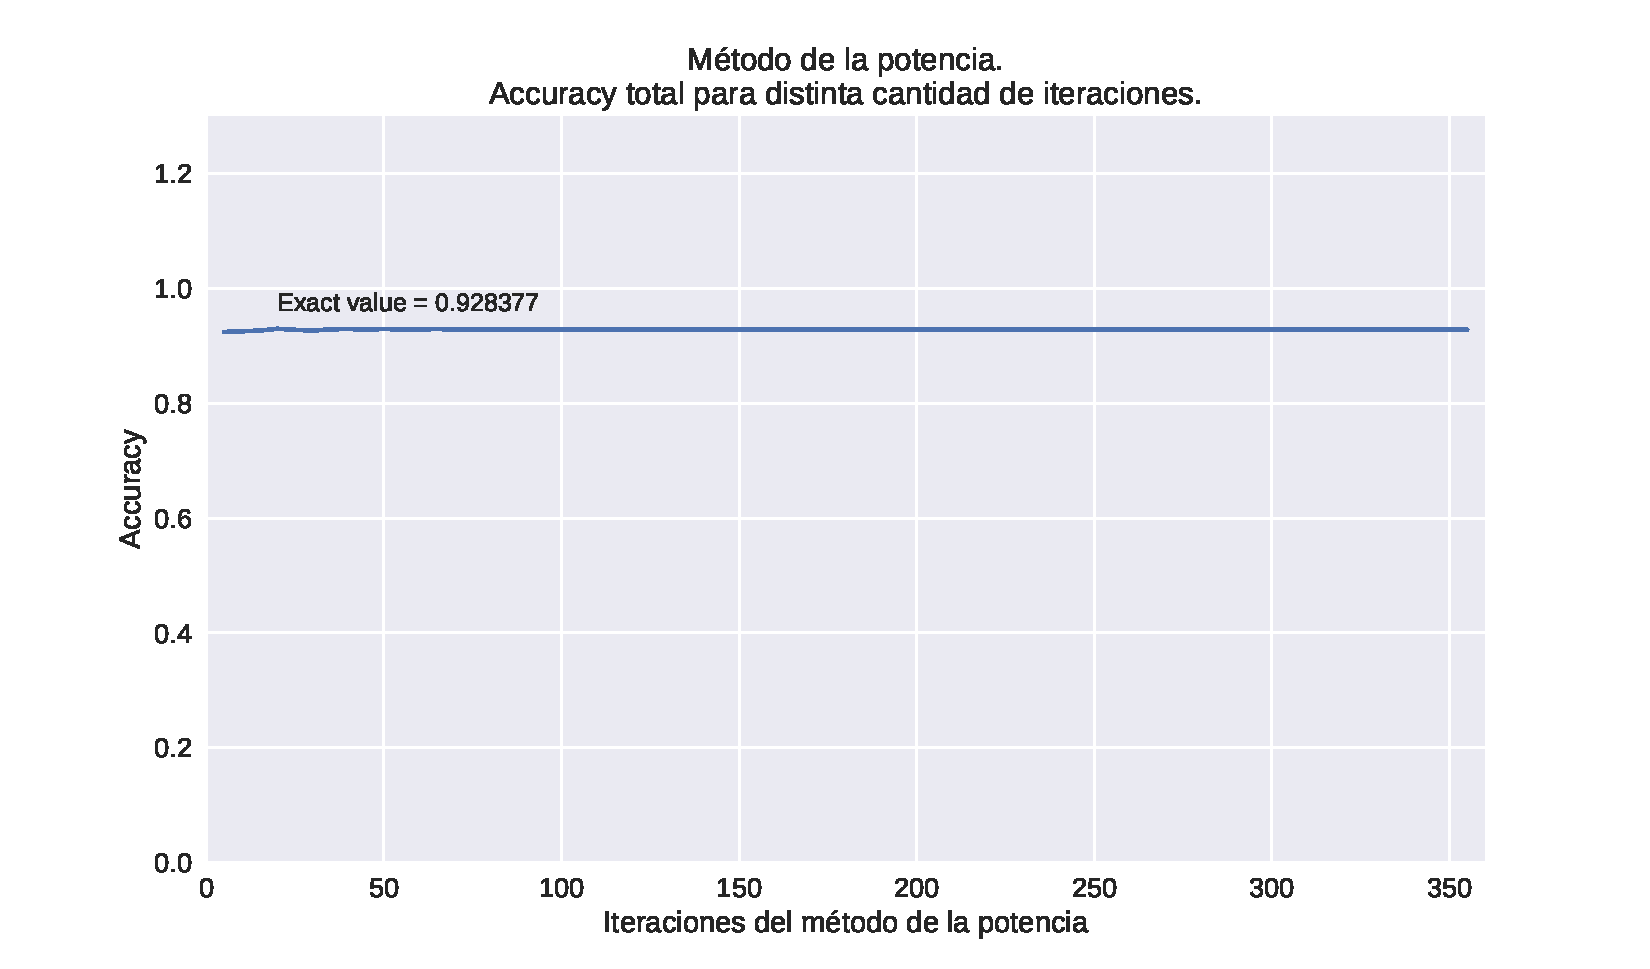
\includegraphics[scale=0.55]{informe/imagenes/potencia/accuracyPorIters.pdf} \\
    \captionof{figure}{Accuracy por cantidad de iteraciones. \\
    Todas las variables fijas \\ }
}
$ $\newline

Como podemos ver, la accuracy se mantiene constante, con la excepción de las cercanías de 10 iteraciones dónde aún son demasiado pocas. Consideramos que no es necesario tomar una cantidad de iteraciones demasiado alta, ya que con aproximadamente 50 parece ser más que suficiente. Es lógico pensar que a mayor cantidad de iteraciones, más tarda nuestro sistema en entrenar. Veamos si el incremento es significativo: \\

{\centering
    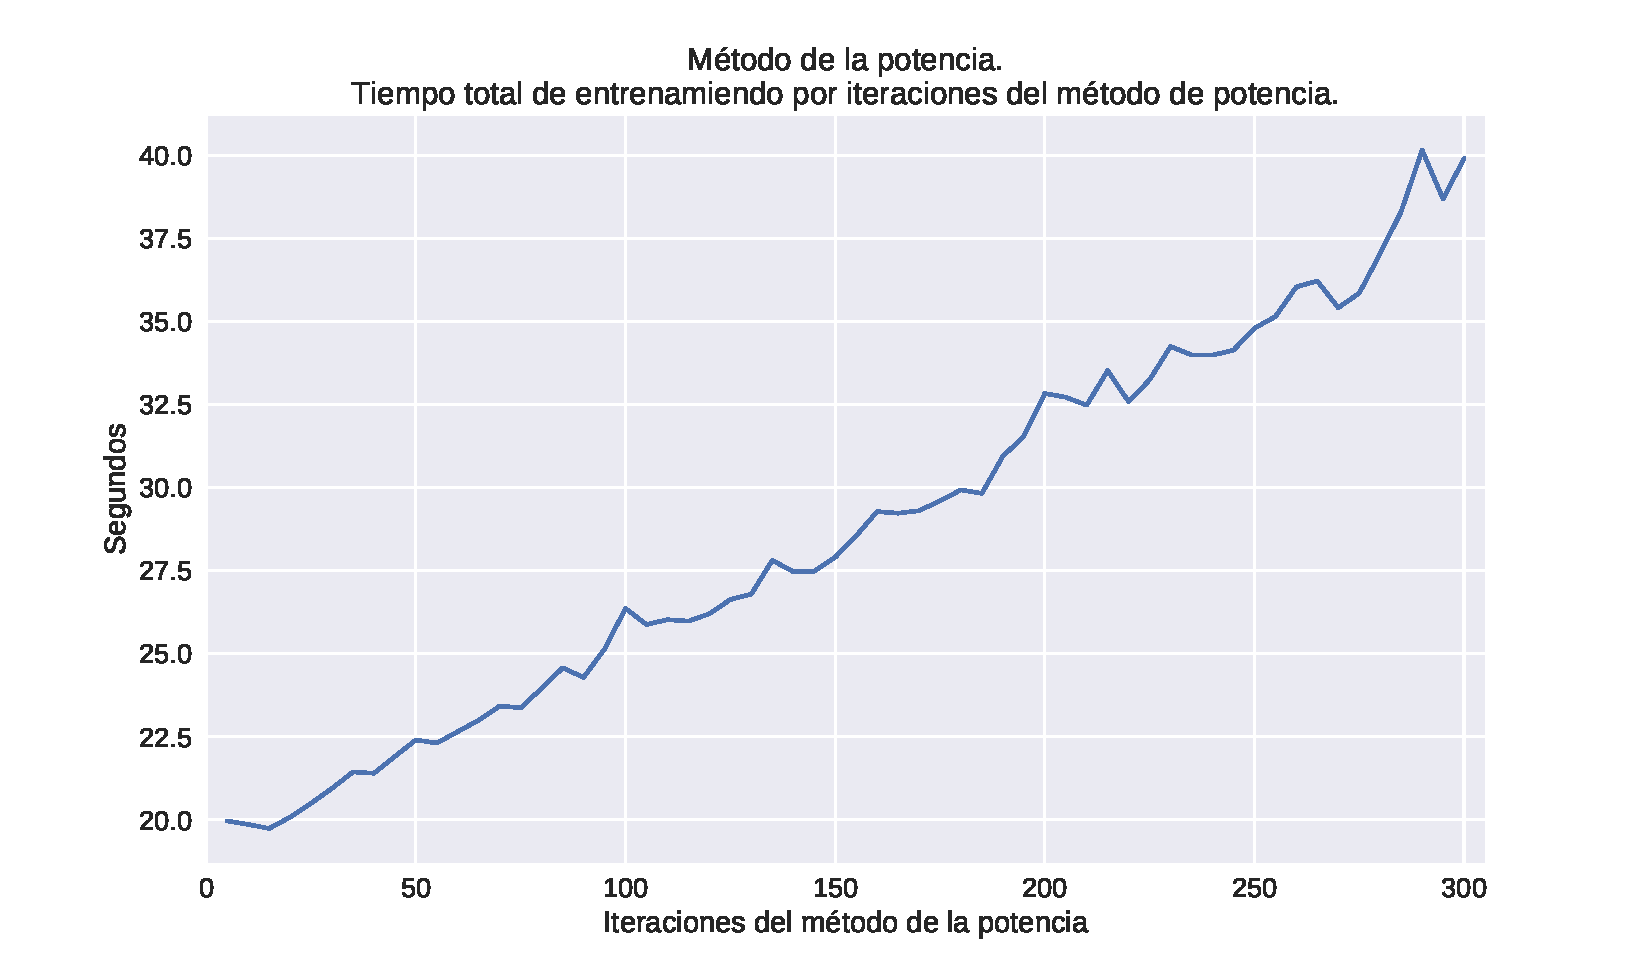
\includegraphics[scale=0.55]{informe/imagenes/potencia/tiempoPorIters.pdf} \\
    \captionof{figure}{Tiempo por cantidad de iteraciones. \\
    Todas las variables fijas \\ }
}
$ $\newline

La diferencia de tiempo es bastante notoria, sobre todo sabiendo que no estamos considerando la cantidad total de datos de entrenamiento. Dado que no encontramos diferencias de accuracy pero sí de tiempo, a partir de ahora fijaremos el parámetro de iteraciones en 50. \\

\subsection{kNN}

\todo[inline]{Quiza, graficar tiempos de knn para 10000 muestras, moviendo el k. Los datos ya estan tomados en knnMediciones, solo hay que extraerlos bien. Creo igual que conviene hacerlo en la comparacion con psa y ya, sino es info repetida-}

Nos gustaría analizar qué tan bien (o qué tan mal) se comporta kNN a medida que vamos variando el \textit{k}. Si bien nuestro espacio posible de muestras es 42000, usar un espacio de ese tamaño se vuelve prohibitivo ya que debemos iterar gran cantidad de veces sobre el espacio. Por este motivo, vamos a considerar un espacio de 10000 muestras. Es esperable que con las 42000 muestras consigamos resultados mejores, y lo verificaremos cuando enviemos los resultados a Kaggle. \\

Dado que nuestros vectores viven en $\mathbb{R}^{784}$, esperamos que los resultados aplicando kNN (sin reducir dimensiones) sean malos por problemas con la \textit{maldición de la dimensión}, y sobre todo porque no estamos considerando el espacio de muestras completo. \\

Sorprendentemente, lo que sucedió es todo lo contrario a lo que esperábamos, y con kNN obtuvimos (en promedio) precisiones de 0.95. \\

La mayoría de las clases se comportan de manera similar, salvo algunas excepciones que veremos más adelante. Veamos por ejemplo la clase del 0, que fue la \textit{mejor} clase.

{\centering
    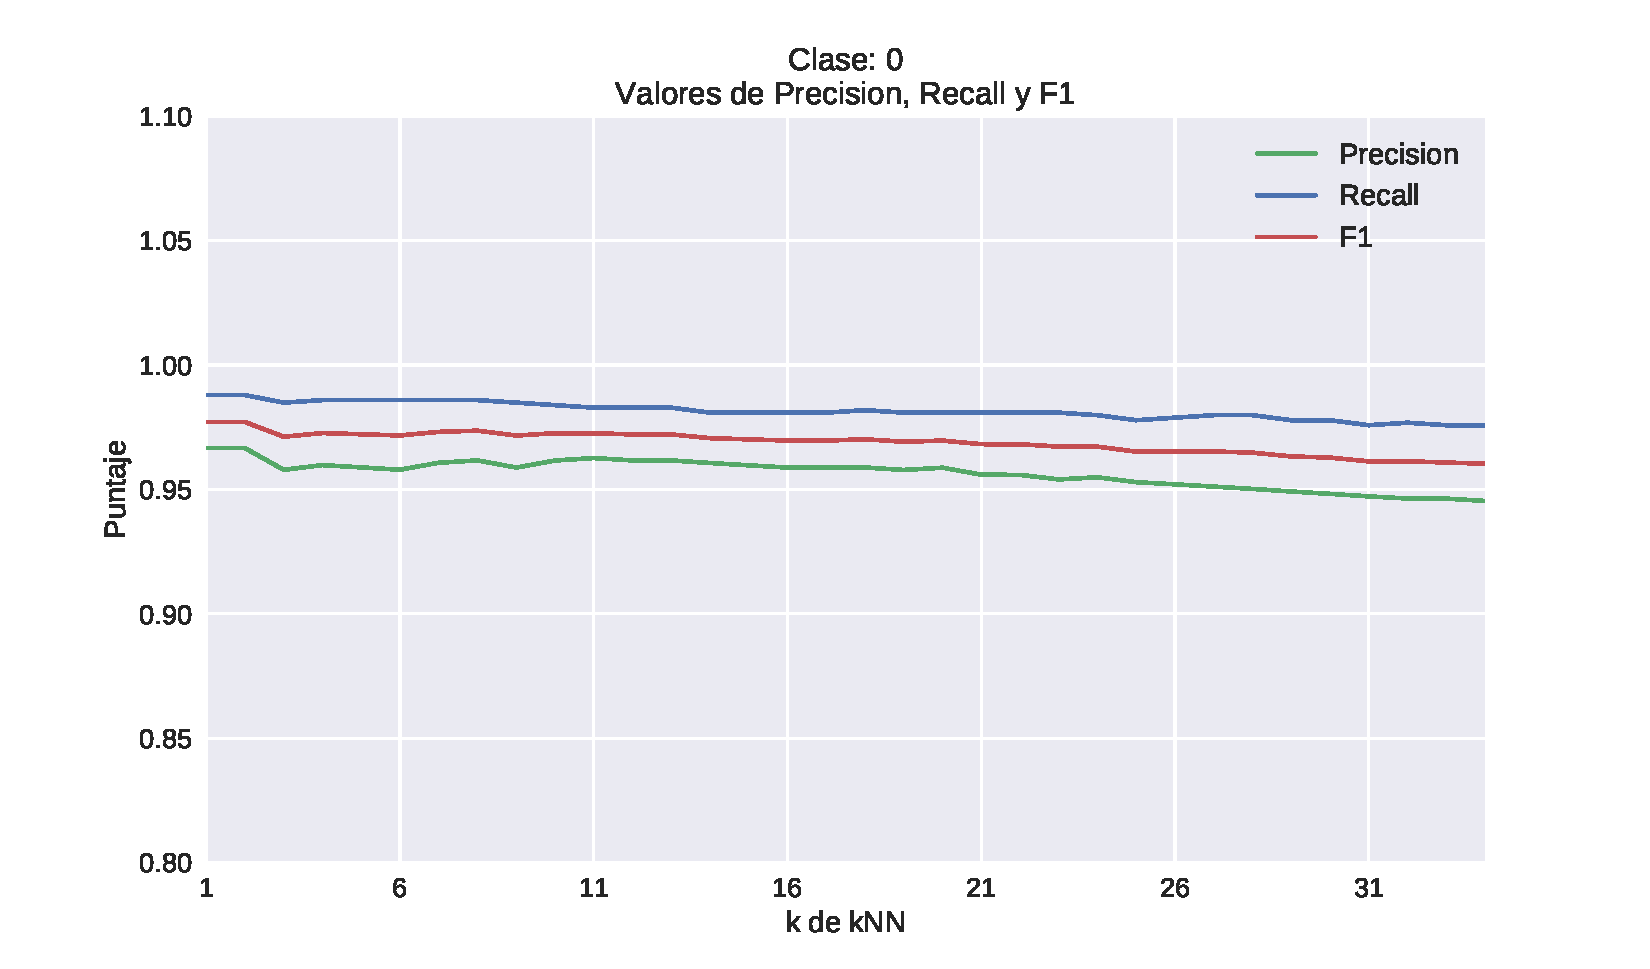
\includegraphics[scale=0.55]{informe/imagenes/knn/precisionClase0.pdf} \\
    \captionof{figure}{Clasificación para clase 0, sólo kNN.\\Precision, Recall y F1, variando k.\\}
}
$ $\newline

Dado que la mayoría de los gráficos son similares, sólo graficaremos a continuación aquellas clases que más se diferencian.

{\centering
    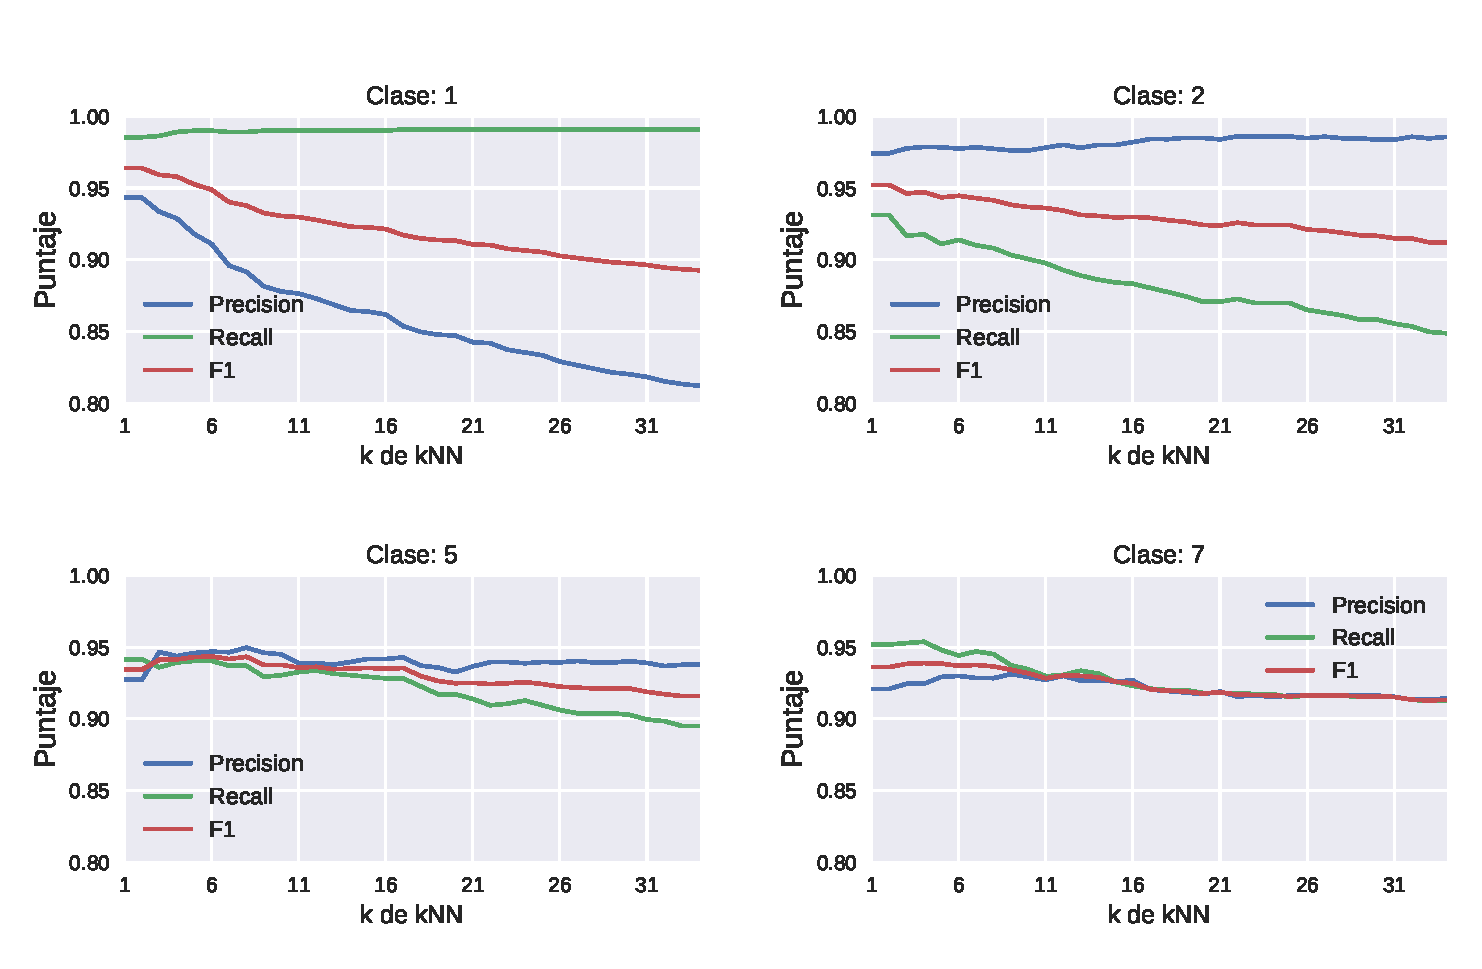
\includegraphics[scale=0.70]{informe/imagenes/knn/precisionClase1257.pdf} \\
    \captionof{figure}{Clasificación para clases 1, 2, 5 y 7, sólo kNN\\Valores de Precision, Recall y F1, variando k.\\}
}
$ $\newline

Lo primero que observamos es lo que nos sorprendió: todos comienzan con un Precision/Recall de aproximadamente 0.95, lo cual es un valor muy alto. Parece ser que pese a los problemas de dimensionalidad y del tamaño de la muestra, kNN se comporta bastante bien. Es esperable que con una muestra más grande se comporte mejor. Veremos más adelante qué dice Kaggle al respecto.\\

Otra cosa que podemos observar, es que a medida que el \textit{k} aumenta, \textit{en general} Precision y Recall disminuyen. Consideramos que este comportamiento tiene sentido ya que por el problema de la dimensionalidad, nuestros vectores estén muy dispersos, entonces con un \textit{k} mas grande los \textit{k} mas cercanos no necesariamente son los de su misma clase. \\

Algo destacable es lo que sucede con la clase del 1 y la clase del 2. Las curvas de Precision y de Recall son opuestas. Si categorizamos una imagen como un 2, es muy probable que sea un 2 realmente. Es decir, cuando lo categorizamos como un 2, no nos equivocamos. Sin embargo, hay muchas imágenes que realmente son 2 pero que no las categorizamos como tal. Con la clase del 1 nos pasa exactamente lo contrario. \\

El objetivo de el experimento era tratar de estimar el mejor \textit{k} para kNN. Nos concentraremos en la curva de F1, pues lo que nos interesa es tener un balance entre Precision y Recall. Buscamos el $k$ tal que F1 llegue a su máximo. Los siguientes son los valores obtenidos: \\

\begin{center}
    \begin{tabular}{| c | c | c | c | c | c | c | c | c | c | c |}
    \hline
    Clase   & 0 & 1 & 2 & 3 & 4 & 5 & 6 & 7 & 8 & 9  \\ \hline
    max_k       & 1 & 1 & 1 & 3 & 4 & 6 & 1 & 4 & 4 & 4  \\ \hline
    \end{tabular}
\end{center}

Sólo podemos quedarnos con un único k, y queremos \textit{favorecer} a todas las clases. Dado que el promedio es 2.9 y la mediana es 3, suponemos que el mejor k es 3. \\

Como habíamos mencionado anteriormente, realizar el mismo experimento con el set completo de datos, sumado a las iteraciones por los folds, nos resulta demasiado costoso. Es por esto que para comprobar la eficacia de nuestro método decidimos probarlo directamente con la competencia de Kaggle. Queremos ver si efectivamente con k = 3 conseguimos el mejor resultado. Los siguientes resultados fueron obtenidos con un entrenamiento de las 42000 imágenes. \\

{\centering
    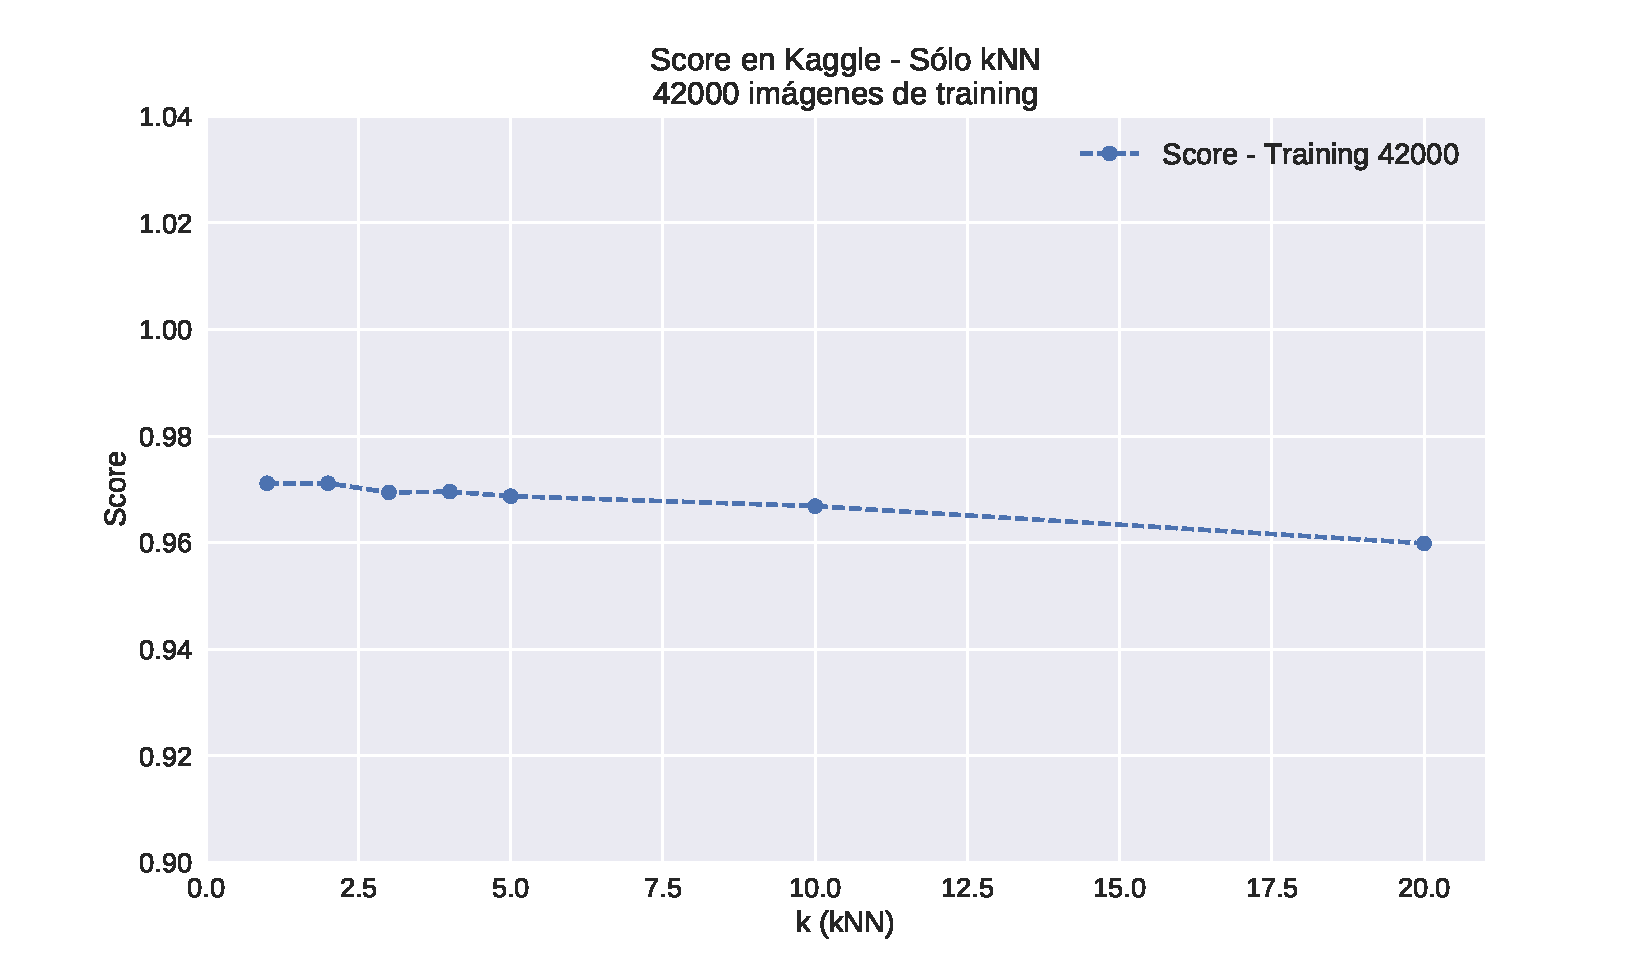
\includegraphics[scale=0.60]{informe/imagenes/knn/kaggleknn.pdf} \\
    \captionof{figure}{Scores competencia de Kaggle variando k.\\Perfil del usuario utilizado: kaggle.com/jonnojs}
}
$ $\newline

Si bien nuestra predicción no fue perfecta, estuvo bastante cerca. Para una mejor apreciación de las diferencias, mostramos un cuadro comparativo con los 4 mejores resultados obtenidos, ordenados por score. \\

\begin{center}
    \begin{tabular}{| c | c |}
    \hline
    % k   & Score  \\ \hline
    % 2   & 0.97114  \\ \hline
    % 4   & 0.96957  \\ \hline
    % 3   & 0.96942  \\ \hline
     Score    & k  \\ \hline
     0.97114  & 1  \\ \hline
     0.97114  & 2  \\ \hline
     0.96957  & 4  \\ \hline
     0.96942  & 3  \\ \hline
    \end{tabular}
\end{center}


En primer lugar, notar que k=1 y k=2 tienen el mismo puntaje. Esto es razonable, si consideramos que con k=2 las posibilidades sobre las clases del primer y segundo mas cercano son las siguientes: \\
\begin{itemize}
\item Si el primero es de clase X y el segundo es de clase X, entonces elegimos clase X
\item Si el primero es de clase X y el segundo es de clase Z, entonces igual nos quedamos con X pues fue el mas cercano.
\end{itemize}

Es decir, k=2 se comporta exactamente igual que no considerar ninguna vecindad. \\

Las diferencias de k=3 con k=2 y k=4 son 0.00172 y 0.00015 respectivamente, que es bastante pequeña considerando la reducción de muestras que hicimos. \\

Aunque los números no mienten, no nos parece intuitivo que no considerar ninguna vecindad sea la mejor opción. Imaginamos que este resultado puede asociarse con la maldición de la dimensionalidad, y creemos que con PSA el mejor k será uno mayor. También es posible que los datos de tests de Kaggle tengan un sesgo hacia aquellos cuyos $k$ óptimo es menor, pero como no conocemos las verdaderas etiquetas no podemos saberlo. \\

\todo[inline]{¿QUIZA? -> Concluimos que para unicamente kNN, el mejor parámetro para k es k=EQUIS.}

\subsection{TODO:}

\todo[inline]{Experimentacion con knn variando los k-knn y los K-folds, para encontrar el mejor parametro posible}

\todo[inline]{Experimentacion de tiempo variando la cantidad de imagenes, no hace falta mil experimentos, un par de puntos clave, digamos 100, 1000, 2000, 5000, 10000, 20000, 40000}

\todo[inline]{Comparacion tiempos con, digamos, 10000 training entre knn a secas y con psa.}

\todo[inline]{Comparacion accuaracy y cosas con, digamos, 10000 training entre knn a secas y con psa.}

\todo[inline]{Podemos variar los K-kfolds si la base de entrenamiento es 'chica'}

\todo[inline]{Para entrenamientos con TODAS las imagenes y PSA, QUIZA nos convenga fijar los kfold en, nose, 5, y solo variar los demas parametros. Es RE costoso, (horas) calcular los K folds con un training grande (CON PSA).  Esta piola la idea de agustin de guardarnos en un txt la matriz de covarianza. \\
En limpio, la idea seria: Para 5 folds calcular y guardar las 5 matrices de covarianza, y despues experimentar variando los alphas y los k-knn. Esto seria 'barato' dentro de todo y podrian hacerce un par de graficos. Si hay tiempo variar el k-KFOLD pero lo dejaria para lo ultimo, mejor conseguir resultados concretos antes.}

\todo[inline]{Al final, mostrar resultados de Kaggle con y sin PSA, ir probando con un par de buenos parametros cuando los obtengamos}

\todo[inline]{Me parece muy piola de probar con manuscritos hechos por nosotros. Solo si sobra tiempo!}